
L'estimation monoculaire de la profondeur est un problème qui consiste à déterminer la distance à la caméra de chaques pixels d'une image en se basant uniquement sur l'image elle-même.

C'est un problème complexe d'actualité avec beaucoup d'application, comme la segmentation des objets ou la reconstruction 3D (pour le cinéma ou pour la modélisation). L'estimation de la profondeur est certe réalisable avec des technologies de prise de vue particulières (comme la stéréovision), mais avec une estimation monculaire transforme n'importe quelle caméra en un capteur de profondeur.

\subsection{Etat de l'art}

Comme expliqué précedemment, du fait de ses applications industrielles direct, ce problème est déjà largement adressé et des modèles de deep learning sont déjà incroyablement performants. Pour ceux proche de notre application on retiendra \textit{DepthAnythingv2} \cite{depthanythingv2}, \textit{Monodepth2} \cite{MonoDepth2}, ou encore \textit{Depth Pro} \cite{depthpro} de apple qui vient tout juste de sortir.

On peut citer aussi \textit{DenseDepth} \cite{DenseDepth} pour de la prédiction sur des images 360°.

\subsection{Choix \& résultat}

Pour la réalisation de ce projet et après les avoir essayé notre choix s'est porté sur \textit{DepthAnythingv2} pour plusieurs raisons. En premier lieu, il faut comprendre que la plupart des modèles d'estimation monoculaire marchent bien sur des champs proches, mais ont tendance à être limité sur des champs lointains. Or ce qui nous interresse, comme nous utilisons des images extérieures à ciel ouvert (souvent), il s'agit souvent de champs lointains et extérieur, ce qui ne correspond pas aux datasets d'entrainement de ces modèles. 

Or justement \textit{depthanythingv2} propose une version "outdoor" et en système métrique, ce qui convient précisément à notre application, notre choix s'est donc porté sur ce modèle et nous avons obtenu des résultats plutôt satisfaisant comme vous pouvez le voir Figure \ref{fig:depth-estimation-exemple}.

\begin{figure}[h!]
    \centering
    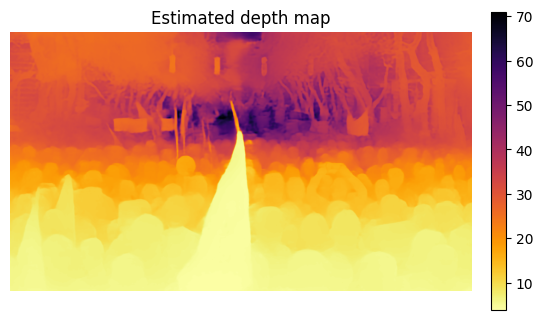
\includegraphics[width=0.45\textwidth]{images/depth_map.png}
    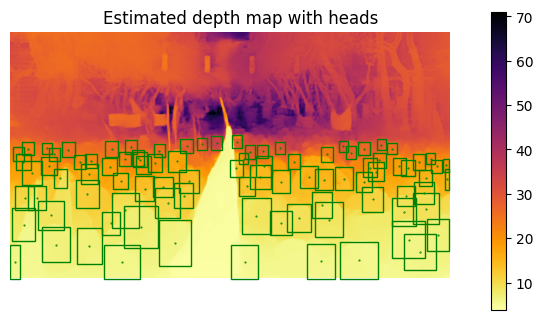
\includegraphics[width=0.45\textwidth]{images/depth_map_with_heads.png}
    \caption{Carte de profondeur estimée par DepthAnythingv2 outdoor (base) sur notre exemple. Sans les headboxes (haut) et avec les headboxes (bas).}
    \label{fig:depth-estimation-exemple}
\end{figure}



